% !TEX root = ../../main.tex
\subsection*{Decision changes occur in short alignments}

The simulation curves include the JC control and the two Tree-of-Life rate-heterogeneous models in the true-tree fixed-length scenario. Under JC, the published and weighted curves coincide, consistent with the repeated non-stationary eigenvalue. Under GTR+F+G4 and LG+G4, decision changes are concentrated in short alignments and long target branches. At 100 sites, the weighted curves remain above the published SatuTe curves at branch lengths 10--12. At 250 sites the separation is smaller, and at 1,000 sites the curves nearly coincide.

\begin{figure}[p]
  \centering
  \makebox[\textwidth][c]{
\includegraphics[width=1.08\textwidth]{figures/figure_power_curve_summary.pdf}}
  \caption{\textbf{Full-alignment simulation curves with and without rate heterogeneity.} Curves show the fraction of replicates called phylogenetically informative in the true-tree fixed-length scenario. The JC panels use 100, 1,000 and 10,000 sites; the GTR+F+G4 and LG+G4 panels use 100, 250 and 1,000 sites. Under JC, the published SatuTe and eigenvalue-weighted curves overlap.}
\end{figure}

The 1,000-replicate grid gives the same interpretation. In the true-tree fixed-length scenario at 100 sites under GTR+F+G4, eigenvalue weighting increased the informative-call fraction by 16.9 percentage points at branch length 10 in the five-taxon case. At branch length 12, the increase was 20.9 percentage points. In the 16-taxon case, the corresponding changes were 22.6 percentage points at both branch lengths. Under LG+G4, the changes were 24.9 and 32.2 percentage points in the five-taxon case. In the 16-taxon case, they were 26.9 and 35.5 percentage points. At 250 sites, the largest changes across these model and tree combinations were 6.5--11.1 percentage points. At 1,000 sites, the two formulas almost always gave the same binary decision.

\subsection*{Decision changes are localized}

The branch-neighborhood analysis tests whether the decision changes are specific to the focal branch. In the 1,000-replicate grid, the difference was concentrated on the target branch. In the true-tree fixed-length scenario at 100 sites and branch length 12, the target-branch change was 14.5 percentage points in the five-taxon GTR+F+G4 case. In the 16-taxon GTR+F+G4 case, it was 22.0 percentage points. The nearest-neighbor change was zero in both cases. Under LG+G4, the corresponding target-branch changes were 38.1 and 39.1 percentage points, again with zero nearest-neighbor change. In these simulations, the weighted statistic changed calls on the tested branch rather than across the surrounding tree.

\begin{figure}[p]
  \centering
  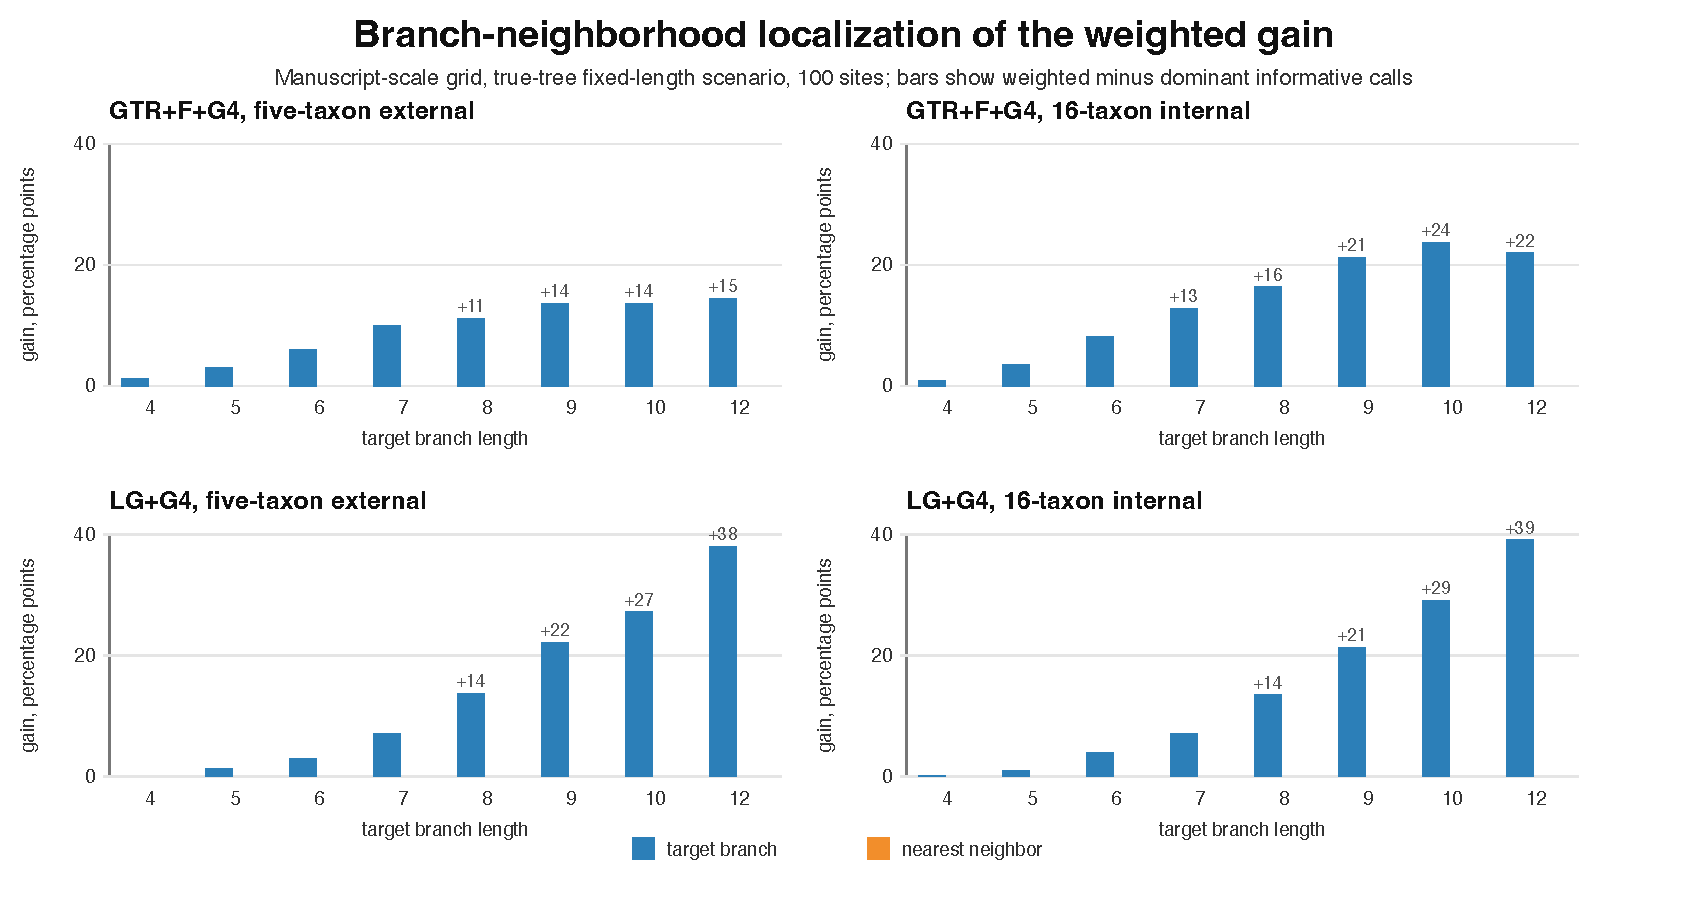
\includegraphics[width=0.98\textwidth]{figures/figure_branch_localization_compact.pdf}
  \caption{\textbf{Branch-neighborhood localization in the 1,000-replicate rate-heterogeneous grid.} Bars show the change in informative-call fraction from eigenvalue weighting at 100 sites in the true-tree fixed-length scenario. The main decision changes occur on the target branch; nearest-neighbor changes are zero in these cells.}
\end{figure}
